% Algebra 2 Lesson 7-2 fast-track packet: Evaluating Trigonometric Functions
% (enVision A2 2024 TE, Example 4 and Example 5 only; draft 2026-10-30, PLC has not met on this lesson)
% Bridge lesson: the special right triangles (45-45-90, 30-60-90) are the SAT-relevant core.
% Shared preamble for the "fast" (hacked-down) Algebra 2 lesson packets, Oct 2026.
% Each packet: % Shared preamble for the "fast" (hacked-down) Algebra 2 lesson packets, Oct 2026.
% Each packet: % Shared preamble for the "fast" (hacked-down) Algebra 2 lesson packets, Oct 2026.
% Each packet: \input{fast-packet-template} then \begin{document} ... \end{document}.
\documentclass[12pt]{article}
\usepackage[margin=0.7in]{geometry}
\usepackage{amsmath,amssymb}
\usepackage{booktabs,tabularx,array}
\usepackage{enumitem}
\usepackage[T1]{fontenc}
\usepackage[utf8]{inputenc}
\usepackage{lmodern}
\usepackage{tikz}
\usepackage{pgfplots}
\pgfplotsset{compat=1.18}
\usepackage{xcolor}
\setlist{nosep,leftmargin=1.4em}
\setlength{\parindent}{0pt}
\setlength{\parskip}{6pt}
\renewcommand{\arraystretch}{1.35}
\newcolumntype{Y}{>{\raggedright\arraybackslash}X}
\pagestyle{empty}

% blanks and workspace
\newcommand{\blank}[1][2.6cm]{\rule[-2pt]{#1}{0.5pt}}
\newcommand{\lines}[1][1]{\par\vspace{2pt}\foreach \i in {1,...,#1}{\rule{0pt}{22pt}\rule{\linewidth}{0.4pt}\par}}
\newcommand{\wspart}[2]{\vspace{4pt}{\large\bfseries #1: #2}\par\vspace{-6pt}\rule{\textwidth}{0.4pt}\par}

% header: \packethead{Lesson 1-3}{Piecewise-Defined Functions}
\newcommand{\packethead}[2]{%
{\LARGE\bfseries #2}\hfill Name \blank[5cm]\\[2pt]
Algebra 2 \quad #1 (fast track) \hfill Date \blank[2.5cm] \quad Period \blank[1.2cm]\par\vspace{2pt}}

% boxed goals: \goals{learning goal}{language goal}
\newcommand{\goals}[2]{%
\fbox{\parbox{\dimexpr\textwidth-2\fboxsep-2\fboxrule}{%
\textbf{Learning goal:} #1\\[2pt]
\textbf{Language goal:} #2}}\par}

% quiz target box: \quiztarget{text}
\newcommand{\quiztarget}[1]{%
\vspace{4pt}\colorbox{gray!12}{\parbox{\dimexpr\textwidth-2\fboxsep}{\textbf{On the quiz:} #1}}\par}

% IXL table row helper: code & skill & which quiz question it feeds
\newcommand{\ixlrow}[3]{\texttt{#1} & #2 & #3 \\}

% one grid style for every graph; override xmin/xmax/... per plot
\pgfplotsset{sheetgrid/.style={
  axis lines=middle, grid=both, grid style={gray!45},
  xmin=-10.5, xmax=10.5, ymin=-10.5, ymax=10.5,
  xtick={-10,-8,...,10}, ytick={-10,-8,...,10},
  x=0.28cm, y=0.28cm,
  ticklabel style={font=\scriptsize, fill=white, inner sep=1pt},
  xlabel={$x$}, ylabel={$y$},
  axis line style={thick}, clip=true}}
% unit grid for small windows
\pgfplotsset{unitgrid/.style={sheetgrid,
  xmin=-5.5, xmax=5.5, ymin=-5.5, ymax=5.5,
  xtick={-5,...,5}, ytick={-5,...,5}, x=0.5cm, y=0.5cm}}
% open and closed endpoints
\tikzset{closed/.style={circle, fill, inner sep=1.6pt},
         open/.style={circle, draw, fill=white, inner sep=1.4pt}}
 then \begin{document} ... \end{document}.
\documentclass[12pt]{article}
\usepackage[margin=0.7in]{geometry}
\usepackage{amsmath,amssymb}
\usepackage{booktabs,tabularx,array}
\usepackage{enumitem}
\usepackage[T1]{fontenc}
\usepackage[utf8]{inputenc}
\usepackage{lmodern}
\usepackage{tikz}
\usepackage{pgfplots}
\pgfplotsset{compat=1.18}
\usepackage{xcolor}
\setlist{nosep,leftmargin=1.4em}
\setlength{\parindent}{0pt}
\setlength{\parskip}{6pt}
\renewcommand{\arraystretch}{1.35}
\newcolumntype{Y}{>{\raggedright\arraybackslash}X}
\pagestyle{empty}

% blanks and workspace
\newcommand{\blank}[1][2.6cm]{\rule[-2pt]{#1}{0.5pt}}
\newcommand{\lines}[1][1]{\par\vspace{2pt}\foreach \i in {1,...,#1}{\rule{0pt}{22pt}\rule{\linewidth}{0.4pt}\par}}
\newcommand{\wspart}[2]{\vspace{4pt}{\large\bfseries #1: #2}\par\vspace{-6pt}\rule{\textwidth}{0.4pt}\par}

% header: \packethead{Lesson 1-3}{Piecewise-Defined Functions}
\newcommand{\packethead}[2]{%
{\LARGE\bfseries #2}\hfill Name \blank[5cm]\\[2pt]
Algebra 2 \quad #1 (fast track) \hfill Date \blank[2.5cm] \quad Period \blank[1.2cm]\par\vspace{2pt}}

% boxed goals: \goals{learning goal}{language goal}
\newcommand{\goals}[2]{%
\fbox{\parbox{\dimexpr\textwidth-2\fboxsep-2\fboxrule}{%
\textbf{Learning goal:} #1\\[2pt]
\textbf{Language goal:} #2}}\par}

% quiz target box: \quiztarget{text}
\newcommand{\quiztarget}[1]{%
\vspace{4pt}\colorbox{gray!12}{\parbox{\dimexpr\textwidth-2\fboxsep}{\textbf{On the quiz:} #1}}\par}

% IXL table row helper: code & skill & which quiz question it feeds
\newcommand{\ixlrow}[3]{\texttt{#1} & #2 & #3 \\}

% one grid style for every graph; override xmin/xmax/... per plot
\pgfplotsset{sheetgrid/.style={
  axis lines=middle, grid=both, grid style={gray!45},
  xmin=-10.5, xmax=10.5, ymin=-10.5, ymax=10.5,
  xtick={-10,-8,...,10}, ytick={-10,-8,...,10},
  x=0.28cm, y=0.28cm,
  ticklabel style={font=\scriptsize, fill=white, inner sep=1pt},
  xlabel={$x$}, ylabel={$y$},
  axis line style={thick}, clip=true}}
% unit grid for small windows
\pgfplotsset{unitgrid/.style={sheetgrid,
  xmin=-5.5, xmax=5.5, ymin=-5.5, ymax=5.5,
  xtick={-5,...,5}, ytick={-5,...,5}, x=0.5cm, y=0.5cm}}
% open and closed endpoints
\tikzset{closed/.style={circle, fill, inner sep=1.6pt},
         open/.style={circle, draw, fill=white, inner sep=1.4pt}}
 then \begin{document} ... \end{document}.
\documentclass[12pt]{article}
\usepackage[margin=0.7in]{geometry}
\usepackage{amsmath,amssymb}
\usepackage{booktabs,tabularx,array}
\usepackage{enumitem}
\usepackage[T1]{fontenc}
\usepackage[utf8]{inputenc}
\usepackage{lmodern}
\usepackage{tikz}
\usepackage{pgfplots}
\pgfplotsset{compat=1.18}
\usepackage{xcolor}
\setlist{nosep,leftmargin=1.4em}
\setlength{\parindent}{0pt}
\setlength{\parskip}{6pt}
\renewcommand{\arraystretch}{1.35}
\newcolumntype{Y}{>{\raggedright\arraybackslash}X}
\pagestyle{empty}

% blanks and workspace
\newcommand{\blank}[1][2.6cm]{\rule[-2pt]{#1}{0.5pt}}
\newcommand{\lines}[1][1]{\par\vspace{2pt}\foreach \i in {1,...,#1}{\rule{0pt}{22pt}\rule{\linewidth}{0.4pt}\par}}
\newcommand{\wspart}[2]{\vspace{4pt}{\large\bfseries #1: #2}\par\vspace{-6pt}\rule{\textwidth}{0.4pt}\par}

% header: \packethead{Lesson 1-3}{Piecewise-Defined Functions}
\newcommand{\packethead}[2]{%
{\LARGE\bfseries #2}\hfill Name \blank[5cm]\\[2pt]
Algebra 2 \quad #1 (fast track) \hfill Date \blank[2.5cm] \quad Period \blank[1.2cm]\par\vspace{2pt}}

% boxed goals: \goals{learning goal}{language goal}
\newcommand{\goals}[2]{%
\fbox{\parbox{\dimexpr\textwidth-2\fboxsep-2\fboxrule}{%
\textbf{Learning goal:} #1\\[2pt]
\textbf{Language goal:} #2}}\par}

% quiz target box: \quiztarget{text}
\newcommand{\quiztarget}[1]{%
\vspace{4pt}\colorbox{gray!12}{\parbox{\dimexpr\textwidth-2\fboxsep}{\textbf{On the quiz:} #1}}\par}

% IXL table row helper: code & skill & which quiz question it feeds
\newcommand{\ixlrow}[3]{\texttt{#1} & #2 & #3 \\}

% one grid style for every graph; override xmin/xmax/... per plot
\pgfplotsset{sheetgrid/.style={
  axis lines=middle, grid=both, grid style={gray!45},
  xmin=-10.5, xmax=10.5, ymin=-10.5, ymax=10.5,
  xtick={-10,-8,...,10}, ytick={-10,-8,...,10},
  x=0.28cm, y=0.28cm,
  ticklabel style={font=\scriptsize, fill=white, inner sep=1pt},
  xlabel={$x$}, ylabel={$y$},
  axis line style={thick}, clip=true}}
% unit grid for small windows
\pgfplotsset{unitgrid/.style={sheetgrid,
  xmin=-5.5, xmax=5.5, ymin=-5.5, ymax=5.5,
  xtick={-5,...,5}, ytick={-5,...,5}, x=0.5cm, y=0.5cm}}
% open and closed endpoints
\tikzset{closed/.style={circle, fill, inner sep=1.6pt},
         open/.style={circle, draw, fill=white, inner sep=1.4pt}}

% unit circle window for every figure in this packet (TE figures: unit circle O, arrowed x/y axes, ticks +/-1)
% Window = TE range +/-1 plus 0.35 padding; grid every half unit (lines at -1, -0.5, 0, 0.5, 1).
% The +/-1 tick labels are suppressed (ticks kept) and printed by \ucirc just outside the circle,
% so no tick label sits on the circle where it crosses an axis.
\pgfplotsset{ucircle/.style={sheetgrid,
  xmin=-1.35, xmax=1.35, ymin=-1.35, ymax=1.35,
  xtick={-1,1}, ytick={-1,1}, minor xtick={-0.5,0.5}, minor ytick={-0.5,0.5},
  xticklabels={}, yticklabels={},
  grid=both, minor grid style={gray!25}, major grid style={gray!45},
  x=1.45cm, y=1.45cm, xlabel={$x$}, ylabel={$y$}, clip=false,
  axis line style={thick, <->},
  every axis x label/.style={at={(axis cs:1.35,0)}, anchor=west, font=\scriptsize},
  every axis y label/.style={at={(axis cs:0,1.35)}, anchor=south, font=\scriptsize}}}
\tikzset{utick/.style={font=\scriptsize, inner sep=1pt}}
\newcommand{\ucirc}{\addplot[thick, domain=0:360, samples=120] ({cos(x)},{sin(x)});
  \node[utick, anchor=north east] at (axis cs:-1,0) {$-1$};
  \node[utick, anchor=north west] at (axis cs:1,0) {$1$};
  \node[utick, anchor=south west] at (axis cs:0,1) {$1$};
  \node[utick, anchor=north west] at (axis cs:0,-1) {$-1$};}
% origin label; the optional argument holds node options (anchor, shifts) so O sits where no arc or ray is drawn
\newcommand{\uO}[1][anchor=north east]{\node[font=\scriptsize, inner sep=0.8pt, #1] at (axis cs:0,0) {$O$};}
\begin{document}

\packethead{Lesson 7-2}{Evaluating Trigonometric Functions}
\goals{I can use special triangles and reference angles to find the values of all six trigonometric functions of an angle in any quadrant.}{I can explain how I found a trigonometric value using the words reference angle, quadrant, terminal point, and reciprocal.}
{\small Spanish: \emph{\'angulo de referencia; secante, cosecante, cotangente; funciones trigonom\'etricas rec\'iprocas}.}

\quiztarget{(1) Sine and cosine of a special angle such as $\frac{2\pi}{3}$ (Example 4). (2) Sine from cosine (full Savvas quiz only). (3) Bonus: which statements about special angles are true, including negative angles and angles past $2\pi$ (Examples 4 and 5). (4) Cosecant, cotangent and secant of $225^\circ$ (Example 5 and the Practice). (5) A point on a radius-8 circle (full Savvas quiz only).}

\wspart{Example 4}{Evaluate Trigonometric Functions with Special Angles as Reference Angles}
\begin{minipage}[t]{0.5\textwidth}
\vspace{0pt}
\begin{enumerate}[label=\textbf{\arabic*.}, itemsep=0pt]
\item Find the \textbf{quadrant} of the terminal side.
\item Find the \textbf{reference angle}: the acute angle between the terminal side and the $x$-axis.
\item A special triangle (hypotenuse 1) gives the legs; the quadrant gives the signs. That is the \textbf{terminal point} $(x,y)=(\cos\theta,\sin\theta)$.
\item $\sin\theta=y$, \ $\cos\theta=x$, \ $\tan\theta=\frac yx$.
\end{enumerate}
\end{minipage}\hfill
\begin{minipage}[t]{0.47\textwidth}
\vspace{0pt}
{\small\textbf{Special triangles, hypotenuse 1} (Example 3)}\par
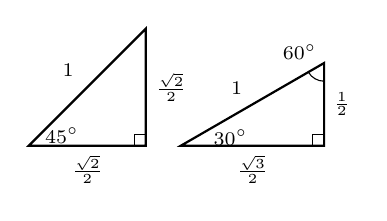
\begin{tikzpicture}[scale=2.1, font=\scriptsize]
\draw[thick] (0,0) -- (0.707,0) -- (0.707,0.707) -- cycle;
\draw (0.637,0) -- (0.637,0.07) -- (0.707,0.07);
\node[above left] at (0.33,0.36) {$1$};
\node[below] at (0.354,0) {$\frac{\sqrt2}{2}$};
\node[right] at (0.707,0.354) {$\frac{\sqrt2}{2}$};
\node at (0.2,0.06) {$45^\circ$};
\begin{scope}[xshift=0.92cm]
\draw[thick] (0,0) -- (0.866,0) -- (0.866,0.5) -- cycle;
\draw (0.796,0) -- (0.796,0.07) -- (0.866,0.07);
\node[above left] at (0.43,0.25) {$1$};
\node[below] at (0.433,0) {$\frac{\sqrt3}{2}$};
\node[right] at (0.866,0.25) {$\frac12$};
\node at (0.3,0.05) {$30^\circ$};
\draw (0.866,0.39) arc[start angle=270, end angle=210, radius=0.11];
\node[anchor=south east, inner sep=1pt] at (0.84,0.5) {$60^\circ$};
\end{scope}
\end{tikzpicture}

{\scriptsize $30^\circ$-$60^\circ$-$90^\circ$: short leg = half the hypotenuse; long leg = short leg $\times\sqrt3$.}
\end{minipage}

\vspace{4pt}
\begin{minipage}[t]{0.32\textwidth}
\raggedright\textbf{A.} What are the sine, cosine, and tangent of $\frac{5\pi}{4}$?\par
\begin{tikzpicture}
\begin{axis}[ucircle, x=1.25cm, y=1.25cm]
\ucirc
\addplot[very thick, red] coordinates {(0,0) (-0.7071,-0.7071)};
\addplot[thick, dashed, blue] coordinates {(-0.7071,-0.7071) (-0.7071,0)};
\addplot[very thick, blue] coordinates {(0,0) (-0.7071,0)};
\addplot[red, ->, domain=0:225, samples=40] ({0.2*cos(x)},{0.2*sin(x)});
\addplot[blue, domain=180:225, samples=20] ({0.42*cos(x)},{0.42*sin(x)});
\node[closed, red] at (axis cs:-0.7071,-0.7071) {};
\node[font=\scriptsize, inner sep=1pt, anchor=north east] at (axis cs:-0.72,-0.74) {$\left(-\frac{\sqrt2}{2},-\frac{\sqrt2}{2}\right)$};
\node[font=\scriptsize, blue, inner sep=0.5pt] at (axis cs:-0.58,-0.19) {$\frac\pi4$};
\node[font=\scriptsize, red, inner sep=0.5pt] at (axis cs:0.36,0.32) {$\frac{5\pi}{4}$};
\uO[anchor=north west]
\end{axis}
\end{tikzpicture}

\small
Quadrant III. Reference angle $\frac{5\pi}{4}-\pi=\frac\pi4$, or $45^\circ$.\\[2pt]
$\sin\frac{5\pi}{4}=-\frac{\sqrt2}{2}$, \ $\cos\frac{5\pi}{4}=-\frac{\sqrt2}{2}$\\[3pt]
$\tan\frac{5\pi}{4}=\dfrac{-\sqrt2/2}{-\sqrt2/2}=1$
\end{minipage}\hfill
\begin{minipage}[t]{0.32\textwidth}
\raggedright\textbf{B.} What are the sine, cosine, and tangent of $330^\circ$?\par
\begin{tikzpicture}
\begin{axis}[ucircle, x=1.25cm, y=1.25cm]
\ucirc
\addplot[very thick, red] coordinates {(0,0) (0.8660,-0.5)};
\addplot[thick, dashed, blue] coordinates {(0.8660,-0.5) (0.8660,0)};
\addplot[very thick, blue] coordinates {(0,0) (0.8660,0)};
\addplot[red, ->, domain=0:330, samples=60] ({0.4*cos(x)},{0.4*sin(x)});
\addplot[blue, domain=330:360, samples=20] ({0.36*cos(x)},{0.36*sin(x)});
\node[closed, red] at (axis cs:0.8660,-0.5) {};
\node[font=\scriptsize, inner sep=1pt, anchor=north west] at (axis cs:0.9,-0.52) {$\left(\frac{\sqrt3}{2},-\frac12\right)$};
\node[font=\scriptsize, blue, inner sep=0.5pt] at (axis cs:0.67,-0.12) {$30^\circ$};
\node[font=\scriptsize, red, inner sep=0.5pt] at (axis cs:-0.45,0.5) {$330^\circ$};
\uO
\end{axis}
\end{tikzpicture}

\small
Quadrant IV. Reference angle $360^\circ-330^\circ=30^\circ$, or $\frac\pi6$.\\[2pt]
$\sin330^\circ=-\frac12$, \ $\cos330^\circ=\frac{\sqrt3}{2}$\\[3pt]
$\tan330^\circ=\dfrac{-1/2}{\sqrt3/2}=-\frac{1}{\sqrt3}=-\frac{\sqrt3}{3}$
\end{minipage}\hfill
\begin{minipage}[t]{0.32\textwidth}
\raggedright\textbf{C.} What are the sine, cosine, and tangent of $\frac{2\pi}{3}$?\par
\begin{tikzpicture}
\begin{axis}[ucircle, x=1.25cm, y=1.25cm]
\ucirc
\addplot[very thick, red] coordinates {(0,0) (-0.5,0.8660)};
\addplot[thick, dashed, blue] coordinates {(-0.5,0.8660) (-0.5,0)};
\addplot[very thick, blue] coordinates {(0,0) (-0.5,0)};
\addplot[red, ->, domain=0:120, samples=30] ({0.2*cos(x)},{0.2*sin(x)});
\addplot[blue, domain=120:180, samples=20] ({0.32*cos(x)},{0.32*sin(x)});
\node[closed, red] at (axis cs:-0.5,0.8660) {};
\node[font=\scriptsize, inner sep=1pt, anchor=south east] at (axis cs:-0.55,0.9) {$\left(-\frac12,\frac{\sqrt3}{2}\right)$};
\node[font=\scriptsize, blue, inner sep=0.5pt] at (axis cs:-0.7,0.2) {$\frac\pi3$};
\node[font=\scriptsize, red, inner sep=0.5pt] at (axis cs:0.36,0.32) {$\frac{2\pi}{3}$};
\uO
\end{axis}
\end{tikzpicture}

\small
Quadrant II. Reference angle $\pi-\frac{2\pi}{3}=\frac\pi3$, or $60^\circ$.\\[2pt]
$\sin\frac{2\pi}{3}=\frac{\sqrt3}{2}$, \ $\cos\frac{2\pi}{3}=-\frac12$\\[3pt]
$\tan\frac{2\pi}{3}=\dfrac{\sqrt3/2}{-1/2}=-\sqrt3$
\end{minipage}

\vspace{4pt}
\textbf{Say it:} The terminal side of $330^\circ$ is in Quadrant \blank[1.2cm], so the reference angle is \blank[1.5cm]. The terminal point is \blank[2.8cm], and $\sin330^\circ$ is negative because \lines[1]

\newpage
\wspart{Try It 4}{Find the sine, cosine, and tangent of angles $\frac{4\pi}{3}$ and $-210^\circ$}
Hint: Sketch each angle and its reference triangle on the unit circle, then fill in the steps. A negative angle turns clockwise.

\begin{minipage}[t]{0.48\textwidth}
\textbf{a.} $\theta=\frac{4\pi}{3}$\par
\begin{minipage}[t]{0.54\linewidth}\vspace{0pt}
\begin{tikzpicture}
\begin{axis}[ucircle, x=1.5cm, y=1.5cm]
\ucirc
\uO
\end{axis}
\end{tikzpicture}
\end{minipage}\hfill
\begin{minipage}[t]{0.44\linewidth}\vspace{8pt}\small
Quadrant: \blank[1.2cm]\\[10pt]
Reference angle:\\[2pt] \blank[1.8cm]\\[10pt]
Terminal point:\\[2pt] $\big(\blank[1.1cm],\ \blank[1.1cm]\big)$
\end{minipage}

\vspace{6pt}
$\sin\frac{4\pi}{3}=\blank[1.6cm]$\qquad $\cos\frac{4\pi}{3}=\blank[1.6cm]$

\vspace{8pt}
$\tan\frac{4\pi}{3}=\blank[1.6cm]$
\end{minipage}\hfill
\begin{minipage}[t]{0.48\textwidth}
\textbf{b.} $\theta=-210^\circ$\par
\begin{minipage}[t]{0.54\linewidth}\vspace{0pt}
\begin{tikzpicture}
\begin{axis}[ucircle, x=1.5cm, y=1.5cm]
\ucirc
\uO
\end{axis}
\end{tikzpicture}
\end{minipage}\hfill
\begin{minipage}[t]{0.44\linewidth}\vspace{8pt}\small
Quadrant: \blank[1.2cm]\\[10pt]
Reference angle:\\[2pt] \blank[1.8cm]\\[10pt]
Terminal point:\\[2pt] $\big(\blank[1.1cm],\ \blank[1.1cm]\big)$
\end{minipage}

\vspace{6pt}
$\sin(-210^\circ)=\blank[1.5cm]$\ \ $\cos(-210^\circ)=\blank[1.5cm]$

\vspace{8pt}
$\tan(-210^\circ)=\blank[1.6cm]$
\end{minipage}

\wspart{Example 5}{Use Reciprocal Trigonometric Identities}
What are the six basic trigonometric functions for angle $\theta$? In addition to sine, cosine, and tangent, there are three more ratios that are defined as \textbf{reciprocal} trigonometric functions.

\begin{minipage}[t]{0.36\textwidth}
\vspace{0pt}
\begin{tikzpicture}
\begin{axis}[ucircle, x=1.65cm, y=1.65cm]
\ucirc
\addplot[very thick, red] coordinates {(0,0) (0.8660,0.5)};
\addplot[thick, dashed, red] coordinates {(0.8660,0.5) (0.8660,0)};
\addplot[very thick, red] coordinates {(0,0) (1.35,0)};
\addplot[red, ->, domain=0:30, samples=20] ({0.4*cos(x)},{0.4*sin(x)});
\node[closed, red] at (axis cs:0.8660,0.5) {};
\node[font=\scriptsize, inner sep=1pt, anchor=south west] at (axis cs:0.9,0.55) {$\left(\frac{\sqrt3}{2},\frac12\right)$};
\node[font=\scriptsize, red, inner sep=0.5pt] at (axis cs:0.52,0.13) {$\theta$};
\uO
\end{axis}
\end{tikzpicture}

{\small Here $\theta=\frac\pi6$ ($30^\circ$).}
\end{minipage}\hfill
\begin{minipage}[t]{0.62\textwidth}
\vspace{0pt}
Cosecant: $\csc\theta=\dfrac1{\sin\theta}=\dfrac1y$ \qquad Secant: $\sec\theta=\dfrac1{\cos\theta}=\dfrac1x$\\[4pt]
Cotangent: $\cot\theta=\dfrac1{\tan\theta}$, also $\cot\theta=\dfrac{\cos\theta}{\sin\theta}=\dfrac xy$

\vspace{6pt}
\begin{tabular}{|l|l|}
\hline
$\sin\theta=\frac12$ & $\csc\theta=\frac21=2$ \\[3pt] \hline
$\cos\theta=\frac{\sqrt3}{2}$ & $\sec\theta=\frac{2}{\sqrt3}\cdot\frac{\sqrt3}{\sqrt3}=\frac{2\sqrt3}{3}$ \\[3pt] \hline
$\tan\theta=\dfrac{\frac12}{\frac{\sqrt3}{2}}=\frac{\sqrt3}{3}$ & $\cot\theta=\frac{3}{\sqrt3}=\frac{3\sqrt3}{3}=\sqrt3$ \\[3pt] \hline
\end{tabular}

\vspace{4pt}
{\small Check: $\cot\theta=\dfrac xy=\dfrac{\frac{\sqrt3}{2}}{\frac12}=\sqrt3$. \checkmark\ A reciprocal has the \textbf{same sign} as its function, so the quadrant signs from Example 4 carry over.}
\end{minipage}

\textbf{Say it:} The secant is the \blank[2.2cm] of the cosine, so for $\theta=\frac\pi6$, $\sec\theta=$ \blank[1.8cm]. To find $\csc\theta$ I use the \blank[1.4cm]-coordinate of the terminal point because \lines[1]

\newpage
\wspart{Try It 5}{Write the six trigonometric functions for the given angle $\theta$}
\begin{minipage}[t]{0.48\textwidth}
\textbf{a.}\par
\begin{minipage}[t]{0.61\linewidth}\vspace{0pt}
\begin{tikzpicture}
\begin{axis}[ucircle, x=1.3cm, y=1.3cm]
\ucirc
\addplot[very thick, red] coordinates {(0,0) (0.3846,-0.9231)};
\addplot[red, ->, domain=0:292.6, samples=60] ({0.22*cos(x)},{0.22*sin(x)});
\node[closed, red] at (axis cs:0.3846,-0.9231) {};
\node[font=\scriptsize, inner sep=1pt, anchor=north west] at (axis cs:0.52,-0.88) {$\left(\frac{5}{13},-\frac{12}{13}\right)$};
\node[font=\scriptsize, red, inner sep=0.5pt] at (axis cs:-0.3,0.3) {$\theta$};
\uO[anchor=north west, xshift=5pt, yshift=-2pt]
\end{axis}
\end{tikzpicture}
\end{minipage}\hfill
\begin{minipage}[t]{0.37\linewidth}\vspace{2pt}
$\sin\theta=\blank[1.5cm]$\\[10pt]
$\cos\theta=\blank[1.5cm]$\\[10pt]
$\tan\theta=\blank[1.5cm]$\\[9pt]
$\csc\theta=\blank[1.5cm]$\\[9pt]
$\sec\theta=\blank[1.5cm]$\\[9pt]
$\cot\theta=\blank[1.5cm]$
\end{minipage}
\end{minipage}\hfill
\begin{minipage}[t]{0.48\textwidth}
\textbf{b.}\par
\begin{minipage}[t]{0.61\linewidth}\vspace{0pt}
\begin{tikzpicture}
\begin{axis}[ucircle, x=1.3cm, y=1.3cm]
\ucirc
\addplot[very thick, red] coordinates {(0,0) (-0.9459,-0.3243)};
\addplot[red, ->, domain=0:198.9, samples=50] ({0.22*cos(x)},{0.22*sin(x)});
\node[closed, red] at (axis cs:-0.9459,-0.3243) {};
\node[font=\scriptsize, inner sep=1pt, anchor=north east] at (axis cs:-0.98,-0.36) {$\left(-\frac{35}{37},-\frac{12}{37}\right)$};
\node[font=\scriptsize, red, inner sep=0.5pt] at (axis cs:0.3,0.3) {$\theta$};
\uO[anchor=north west]
\end{axis}
\end{tikzpicture}
\end{minipage}\hfill
\begin{minipage}[t]{0.37\linewidth}\vspace{2pt}
$\sin\theta=\blank[1.5cm]$\\[10pt]
$\cos\theta=\blank[1.5cm]$\\[10pt]
$\tan\theta=\blank[1.5cm]$\\[9pt]
$\csc\theta=\blank[1.5cm]$\\[9pt]
$\sec\theta=\blank[1.5cm]$\\[9pt]
$\cot\theta=\blank[1.5cm]$
\end{minipage}
\end{minipage}

\vspace{2pt}
In part a, why is $\csc\theta$ negative? Use the words \emph{terminal point} and \emph{reciprocal}.\lines[2]

% R5: rehearses Savvas Lesson Quiz item 4 (csc, cot and sec of 225 degrees: a special angle outside
% Quadrant I, then reciprocals). Neither Try It does both steps. This block is TE Practice & Problem
% Solving 14 (Error Analysis, SEE EXAMPLE 5) plus Concept Summary "Do You Know How" 11 (135 degrees),
% not the quiz item. Key: sec 135 = -sqrt2 (the TE prints +sqrt2 for item 14; -sqrt2 is correct),
% csc 135 = sqrt2, cot 135 = -1.
\wspart{Practice}{Reciprocals of a special angle outside Quadrant I}
\textbf{a.} Describe and correct the error a student made in evaluating the secant of a $135^\circ$ angle.

\begin{center}
\fbox{\parbox{0.8\textwidth}{\small The coordinates of the terminal point on the unit circle are $\left(-\frac{\sqrt2}{2},\frac{\sqrt2}{2}\right)$.\\[4pt]
\hspace*{3cm}$\sec135^\circ=\dfrac{-\frac{\sqrt2}{2}}{1}=-\dfrac{\sqrt2}{2}$ \quad {\color{red}\large$\times$}}}
\end{center}
\lines[2]

\textbf{b.} Find the secant, cosecant, and cotangent of a $135^\circ$ angle.

{\small Hint: Quadrant? Reference angle? Terminal point? Then take reciprocals.}

$\sec135^\circ=\blank[2cm]$\qquad $\csc135^\circ=\blank[2cm]$\qquad $\cot135^\circ=\blank[2cm]$
\lines[2]

\newpage
\wspart{IXL}{Practice for the quiz}
Go to IXL, Algebra 2. Type the code in the search box. Do the starred skills first.
\textbf{SmartScore 70 or above on each starred ($\bigstar$) skill replaces your quiz score.}

\vspace{2pt}
\begin{tabularx}{\textwidth}{l Y Y}
\toprule
\textbf{Code} & \textbf{Skill} & \textbf{Feeds} \\
\midrule
\ixlrow{6H8 $\bigstar$}{Evaluate trigonometric ratios using reference angles: sin, cos, tan}{Quiz 1; Quiz 3 bonus (Example 4)}
\ixlrow{PAE $\bigstar$}{Evaluate trigonometric ratios using reference angles: sec, csc, cot}{Quiz 4; Quiz 3 bonus (Example 5)}
\ixlrow{ZF7}{Determine trigonometric ratios using points on the unit circle (optional)}{Try It 5 only: six functions from a terminal point; no scored quiz item}
\ixlrow{NUF}{Special right triangles}{Warm-up: the $45^\circ$ and $30^\circ$-$60^\circ$ legs}
\ixlrow{BRP}{Reference angles}{Warm-up: step 2 of Example 4}
\bottomrule
\end{tabularx}

% R3 no-DOK-3 rule: the TE item analysis prints no DOK 3 for 7-2 (DOK 1 and 2 only), so the Exit block carries the hardest item tied to a kept Example.
% Kept: TE Practice & Problem Solving 19 (Error Analysis, DOK 2, Example 4 in the item analysis).
% Key: tan(theta) = sin/cos = (4/5)/(-3/5) = -4/3; the student wrote cos/sin, the reciprocal (cotangent).
\wspart{Exit question}{Practice 19 (Error Analysis)}
\fbox{\parbox{\dimexpr\textwidth-2\fboxsep-2\fboxrule}{\raggedright
If the coordinates of the terminal point of an angle $\theta$ on the unit circle are $\left(-\frac35,\frac45\right)$, describe and correct the error a student made in finding $\tan\theta$.

\begin{center}
\fbox{\small $\tan\theta=\dfrac{-\frac35}{\frac45}=-\dfrac34$ \quad {\color{red}\large$\times$}}
\end{center}
\lines[3]
The terminal point is $(x,y)=\big(\blank[1.2cm],\ \blank[1.2cm]\big)$, in Quadrant \blank[1.2cm]. The student divided \blank[2cm] by \blank[2cm], which gives the \blank[2.6cm] of the tangent (the cotangent). The correct value is $\tan\theta=\dfrac yx=$ \blank[2cm].
}}

\vspace{6pt}
\textbf{Before the quiz, finish these sentences.}

The terminal point of $\theta$ on the unit circle is $\big(\blank[1.6cm],\ \blank[1.6cm]\big)$.

The reference angle is the acute angle between the terminal side and the \blank[2.5cm].

The \blank[2.5cm] of the terminal side tells me the signs of $\sin\theta$ and $\cos\theta$.

$\csc\theta$, $\sec\theta$ and $\cot\theta$ are the \blank[2.5cm] of $\sin\theta$, $\cos\theta$ and $\tan\theta$.

\end{document}
